% !TEX root = ./paper.tex
% Design note to remember to explain: multi-stream \tcpls must increase the lower
% 64 bits of the IV to keep using a counter starting a 0. (though, we need a
% limit on the number of paralel stream creation)

\vspace{-0.1cm}
\subsection{The Secure Control Channel}\label{sec:extending}

\texttt{TLS 1.3}~\cite{rfc8446} has been designed with careful consideration for
potential extensions. It supports the EncryptedExtensions message sent by the
server alongside the ServerHello. Any extension sent with the ServerHello
message is
encrypted with the handshake key, and is not part of the context used
to derive the eventual application key.
%Such a design choice eases dealing with implementations
%not supporting a particular option since an opportunistic transmission
%of an option will not affect the handshake outcome.

A reasonable approach to designing extensibility mechanisms in today's
Internet is to avoid leaking any information that could help an
on-path attacker recognize specific users or applications.
Indeed, censorship~\cite{Morshed2017a, Gosain2017a,Chai2019a} can be easily implemented when protocol messages
can be distinguished, and avoiding trivial
opportunities to implement censorship should become the bare minimum in
designing a new protocol. \tcpls's control protocol considers those problems by
avoiding unencrypted data within the ClientHello.

In our design, the client indicates its willingness to use \tcpls
with a transport parameter in the ClientHello. Upon reception of this parameter,
the server can
opportunistically send lightweight \tcpls data and \tcp options as
EncryptedExtensions. If the client does not support some extension, it
echoes back an alert with the value of the option it does not recognize, but
the connection continues.

The server or the client can also send \tcpls control messages
after the handshake. These control messages
take advantage of the \texttt{TLS 1.3} content-type extensibility feature
to avoid
middlebox interference. Indeed, in \texttt{TLS 1.3}, the Record Protocol
ensures that any new message appears as an \texttt{APPDATA} message type
while the true content type (TType) is stored at the end of the encrypted payload.
As an example, Figure~\ref{ex_record}
shows the \tcpls control message structure that carries the
\tcp User Timeout~\cite{rfc5482} option. $TType$ is the true type of this
record (TCP\_OPTION), while its  Type is set to $APPDATA$.

% Discussing the lack of extensibility of TLS 1.3;
\begin{figure}
  \begin{bytefield}[bitwidth=0.47em]{40}
    \bitheader[lsb=0,bitformatting={\tiny\rotatebox[origin=B]{90}}]{0-39} \\
    \begin{rightwordgroup}{Header}
      \bitbox{8}{Type} & \bitbox{16}{Version} & \bitbox{16}{Length}
    \end{rightwordgroup}\\
    \begin{rightwordgroup}{Payload}
      \bitbox{16}{Option Type} & \bitbox{16}{User Timeout} & \bitbox{8}{TType}
     %&\wordbox[lrb]{1}{Padding... (to match the AEAD block size)}
    \end{rightwordgroup}\\
  \end{bytefield}
  \caption{A new type of TLS Record containing a \tcp option.}
  \label{ex_record}
\end{figure}


\subsection{Datastreams and \tcp Connections}
\label{sec:datastreams}

In \tcpls, each stream has its own cryptographic
context. They use the same key but derive the blockcipher IV such that
nonce-misuse cannot happen while the record sequence number within each stream
starts at 0. Only one application-level key is used for N streams, for each direction.
The reason behind this design choice is to avoid security degradation with the
usage of multiple keys (by a factor $k$ with $k$
keys)~\cite{chatterjee2011another}.

Having a separate cryptographic
context means that \tcpls can do concurrent encryption and decryption
between streams while maintaining decryption correctness and security, and potentially also use this
capability to process streams over multiple cores. Finally, if we have multiple
streams over the same \tcp connection, \tcpls does not explicitely know which received data belongs to
which stream. To obtain this information, we either require to modify the
associated information within  \tls records to add a stream id (these associated
data are not encrypted but the AEAD cipher authenticates them). This
choice means potential middlebox interference, which we chose to avoid. The other option
is to leverage the AEAD cipher to check the authentication tag of the incoming
record until we find the stream that properly verifies the tag). This operation is
lightweight: it does not require full decryption of the record because
\texttt{TLS 1.3}
uses AEAD ciphers doing Encrypt then MAC (and MAC then
Decrypt), and looking for the right stream needs to be performed once each time
the application writes to another stream over the same \tcp connection.

Note that, security-wise, each failed decryption is considered as a
forgery attempt. However, we have large limits on the confidentiality and
integrity with all AEAD ciphers~\cite{luykx2015limits, aeadlimits} before a
successful iorgery may be considered as a non-negligeable probability.

%Streams are an interesting abstraction for applications. Experience with HTTP/2
%has shown that head-of-line blocking was an important factor in web performance.
%This motivated the first QUIC design \cite{langley2017quic}. If all data streams
%are mapped on the same underlying \tcp connection, head-of-line blocking remains
%possible. However, this blocking can be prevented by using different \tcp
%connections to transport the different data streams.

\tcpls enables the client
or the server to associate new \tcp connections to an existing \tcpls
connection. This is similar to what Mutipath \tcp does \cite{raiciu2012hard,rfc6824},
but with some differences. First, Multipath TCP supports only one bytestream.
Second, \tcpls does not suffer from the same security limitations as Multipath
TCP. To secure the attachment of additional subflows, Multipath TCP hosts
exchange keys in plaintext during the handshake \cite{rfc6824, rfc8684}.
These keys are
then used later to authenticate the attachment of subflows to a connection. An
attacker that has observed the initial handshake can attach any subflow to an
existing Multipath TCP connection \cite{rfc6181}.

\tcpls securely solves this \texttt{"connection join"} problem. For example, consider a
client connecting to a dual-stack server. Figure~\ref{fig:join-example} depicts
the \tls messages exchanged.  The client starts with a ClientHello. This includes
the \tcpls extension to negotiate \tcpls. The server replies with a ServerHello
containing several important and encrypted control information $\alpha$. First, the server announces
its IPv4 and IPv6 addresses. Second, it associates one connection identifier.
This identifier uniquely identifies the connection on the server. Third, the
server provides a list of cookies that enable the client to attach additional
\tcp connections to the \tcpls connection. To attach a new connection, e.g., using
the server's IPv6 address, the client opens a \tcp connection and sends a
ClientHello message containing the connection identifier ($CONNID$) and one of the cookies
supplied ($COOKIE$) by the server.

The Connection identifier allows the server to attach the new \tcp connection to
the right \tcpls session, assuming the received cookie is valid. The Connection
identifier and the cookie
play that same role as Multipath TCP's token. However, the cookie is longer, encrypted in
the ServerHello message, and one-time use (i.e., when the server receives a valid
cookie, it accepts the connection, attaches it to the right \tcpls session, and
discard the cookie). Thanks to the cookies, the server can
limit the number of \tcp connections that a client can attach to a \tcpls
connection.
This prevents some denial of service attacks that are
possible with Multipath TCP.

\begin{figure}
  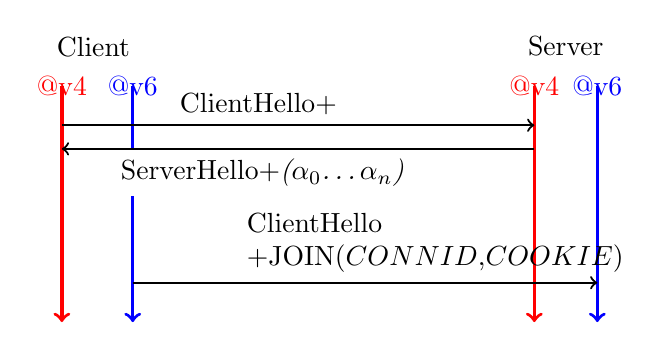
\begin{tikzpicture}
    \colorlet{lightgray}{black!20}
    \tikzstyle{arrow} = [thick,->,>=stealth]
    \tikzset{state/.style={rectangle, dashed, draw, fill=white} }
    \node[black, fill=white] at (0,10) {Client};
    \node[black, fill=white] at (6,10) {Server};
    \node[red, fill=white] at (5.6,9.5) {@v4};
    \node[blue, fill=white] at (6.4,9.5) {@v6};
    \node[red, fill=white] at (-0.4,9.5) {@v4};
    \node[blue, fill=white] at (0.5,9.5) {@v6};
    \draw[red, very thick,->] (-0.4,9.5) -- (-0.4,6.5);
    \draw[blue, very thick,->] (0.5,9.5) -- (0.5,6.5);
    \draw[red, very thick,->] (5.6,9.5) -- (5.6,6.5);
    \draw[blue, very thick,->] (6.4,9.5) -- (6.4,6.5);
   \draw[black, thick, ->] (-0.4,9) -- (5.6,9) node [midway, fill=white, above,
   text width=3cm]
   {ClientHello+\emph{\tcpls}};
   \draw[black, thick, <-] (-0.4,8.7) -- (5.6,8.7) node [midway, fill=white, below,
   text width=4.5cm] { ServerHello+\emph{\tcpls($\alpha_0$\ldots$\alpha_n$)} };
   \draw[black, thick, ->] (0.5,7) -- (6.4,7) node [midway, fill=white, above,
   text width=3cm]
   {ClientHello\\+JOIN($CONNID$,$COOKIE$)};
  \end{tikzpicture}

  \caption{\tcpls supports the attachment of additional \tcp
    connections to a \tcpls connection. Each $\alpha_i$ is encrypted with the
    handshake key.}
  \label{fig:join-example}
\end{figure}

\subsection{The \tcpls API}

The API that applications use to interact with a protocol plays an important
role in enabling them to leverage all the protocol features. The most
popular API to interact with the transport layer remains the BSD socket
API. Researchers and the IETF have explored new
ways to expose a transport API~\cite{draft-ietf-taps-arch,hruby2014sockets,rfc6458,hesmans2016enhanced,schmidt2013socket}.

In this spirit, application-level developers would only be required to
configure a \texttt{\tcpls} context and register function callbacks.
%We design \tcpls such
%that the application-level developers can ignore any notion of Network IPC as
%defined by, for example, the POSIX API, the Berkeley socket API or Winsock,
%facilitating application-level development by offering a more concrete
%session-level interface based on asynchronous network events.
%The overall idea is to offer to application developers the opportunity to tune
%the transport protocol for a better usage of the network from their own
%application protocol, which might depend on its distinguishing
%features.
%\todo{we need to explain the mpjoin}
To illustrate \tcpls API's flexibility, we consider a simple
use case inspired by Happy Eyeballs \cite{rfc8305}. This technique is
used by web browsers when interacting with dual-stack servers. They
try to establish \tcp connections using IPv4 and IPv6 and prefer the
one that offers the lowest latency. This avoids problems when an address
family is broken on a path but not the other and sometimes results in
lower latency \cite{bajpai2019longitudinal}.


\begin{figure}[t]
  \resizebox{0.49\textwidth}{!}{%
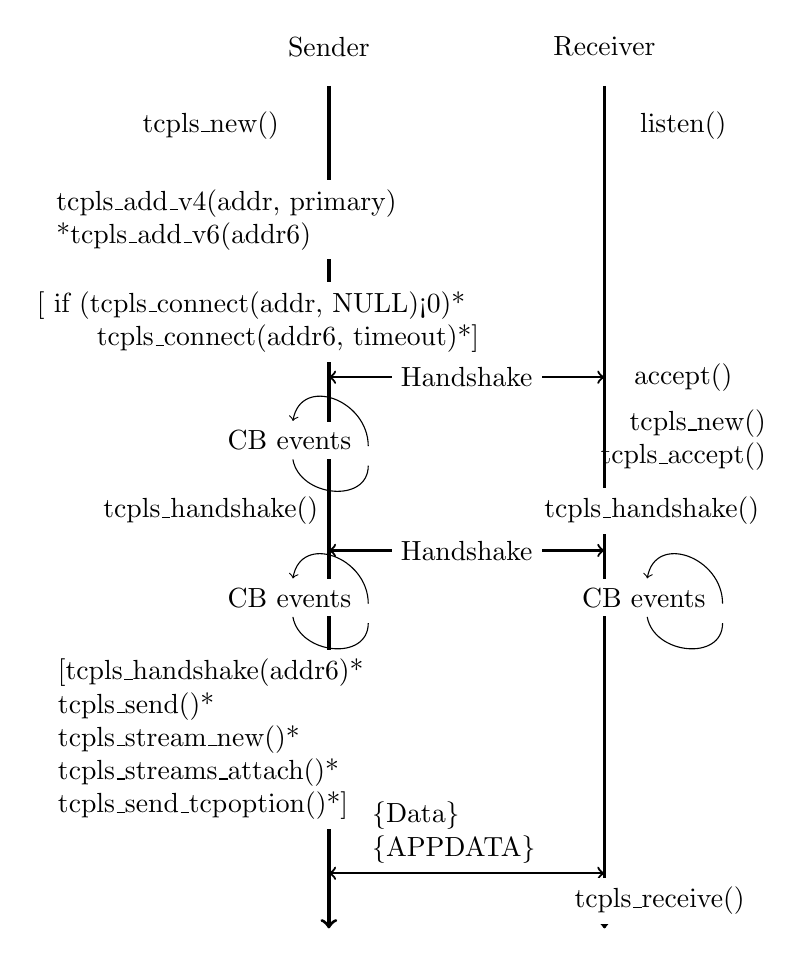
\begin{tikzpicture}
   \colorlet{lightgray}{black!20}
   \tikzstyle{arrow} = [thick,->,>=stealth]
   \tikzset{state/.style={rectangle, dashed, draw, fill=white} }
   \node[black, fill=white] at (0.5,10) {Sender};
   \node[black, fill=white] at (4,10) {Receiver};
   \draw[very thick,->] (0.5,9.5) -- (0.5,-1.2);
   \draw[very thick,->] (4,9.5) -- (4,-1.2);
   \node at (-1,9) {tcpls\_new()};
   \node at (5, 9) {listen()};
   \node[align=left, fill=white] at (-0.8,7.8) {tcpls\_add\_v4(addr,
     primary)\\*tcpls\_add\_v6(addr6)};
   \node[fill=white, align=left] at (-0.4,6.5) {[ if (tcpls\_connect(addr,
     NULL)<0)*\\
     \indent~~tcpls\_connect(addr6, timeout)*]};
   \draw[black, thick, <->] (0.5,5.8) -- (4,5.8) node [midway, fill=white] {\tcp Handshake};
   \node[fill=white] at (0,5) (Callback) {CB events};
   \node at (1,4.8) (here) {};
   \draw [->] (Callback) to[out=-80, in=-90,looseness=1.3] (here)
   to[out=90,in=80,looseness=1.5] (Callback);
   \node at (5, 5.8) {accept()};
   \node[align=right] at (5, 5) {tcpls\_new()\\tcpls\_accept()};
   \node at (-1,4.1) {tcpls\_handshake()};
   \node[fill=white] at (4.6,4.1) {tcpls\_handshake()};
   \draw[black, thick, <->] (0.5,3.6) -- (4,3.6) node [midway, fill=white] {\tcpls Handshake};
   \node[fill=white] at (0,3) (CB2) {CB events};
   \node at (1,2.8) (here2) {};
   \draw [->] (CB2) to[out=-80, in=-90,looseness=1.3] (here2)
   to[out=90,in=80,looseness=1.5] (CB2);
   \node[fill=white] at (4.5,3) (CB3) {CB events};
   \node at (5.5,2.8) (here3) {};
   \draw [->] (CB3) to[out=-80, in=-90,looseness=1.3] (here3)
   to[out=90,in=80,looseness=1.5] (CB3);
   \node[fill=white, align=left] at (-1, 1.2)
   {[tcpls\_handshake(addr6)*\\tcpls\_send()*\\tcpls\_stream\_new()*\\tcpls\_streams\_attach()*\\tcpls\_send\_tcpoption()*]};
   \draw[black, thick, <->] (0.5,-0.5) -- (4,-0.5) node [midway, fill=white,
   above, text width=2.4cm]
   {\{\tcpls Data\} \{APPDATA\}};
   \node[fill=white] at (4.7,-0.85) {tcpls\_receive()};
\end{tikzpicture}
}
\caption{API Workflow example. * means optional call, [ ] means optional call flow, and \{
  \} means encrypted.}
  \label{fig:api}
\end{figure}

Figure~\ref{fig:api}
shows an example of our current API workflow. The API can handle
explicit multipath techniques such as Happy Eyeball by chaining
\texttt{tcpls\_connect()} with an appropriate timeout of 50ms, as shown in the
Figure. \tcpls lets the application explicitly choose
the multipath mesh by calling several times \texttt{tcpls\_connect(src, dest,
  timeout)};. The application may configure callbacks to connection events that
would occur within \tcpls, such as a connection establishment, a stream
attachment, a multipath join, the reception of a \tcp option to tune TCP, and
more. When
multiple streams are attached to multiple \tcp connections, the application may
configure various \tcpls behaviours. Among them, we support HOL-blocking avoidance, aggregation of
bandwidth with multipathing, connection failover, and connection migration.
Note that, HOL-blocking avoidance is incompatible with the aggregation of bandwidth
with multipathing (the application can do either one but not both at the same
time).

\subsection{Comparison to QUIC, \tcp and \tls/\tcp}

Table~\ref{table:tcplsvsquic} compares the features supported by
\tcp, \tls/\tcp, QUIC and \tcpls. QUIC and \tcpls are very similar in their
capabilities. They mainly differ in their semantic. \tcpls's semantic is to let
the applications make the decision, and we design its API to fulfill this goal.
That is, the meaning of \tcpls is to offer advanced, extensible and secure
transport-layer functionalities on top of \tcp, while exposing a simple but
powerful API to let the application composes the properties its transport should
have. One example is further demonstrated in Section~\ref{sec:connmigr}, in
which \tcpls's simple API allows the application to take advantage of path
aggregation (in multipath mode) and connection migration to obtain
a smooth handover between networks.

Note that several of the features suggested by \tcpls are also suggested on \tcp or
QUIC via research works such as a new socket API for explicit multipath for
\tcp\cite{hesmans2016enhanced}, or eBPF plugins in
QUIC~\cite{de2019pluginizing}.

\begin{table}
  \small
  \begin{tabular}{lcccc}
    \toprule
    & \tcp & \tls/\tcp & QUIC & \tcpls \\
    \midrule
    Transport reliability & \checkmark & \checkmark &
    \checkmark & \checkmark \\
    Message conf. and auth.&  \xmark & \checkmark & \checkmark & \checkmark \\
    Connection reliability &  \xmark & \xmark & \checkmark & (\checkmark) \\
    0-RTT & \checkmark & (\xmark) & \checkmark  & \checkmark \\
    Session Resumption & \xmark & \checkmark & \checkmark & \checkmark \\
    Connection Migration & \xmark & \xmark & \checkmark & \checkmark \\
    \multicolumn{5}{l}{Application-exposed features} \\
    \hspace{2em} Streams & \xmark & \xmark & \checkmark & \checkmark \\
    \hspace{2em} Happy eyeballs & \xmark & \xmark & \xmark & \checkmark \\
    \hspace{2em} Explicit Multipath & \xmark & \xmark & \xmark & \checkmark \\
    \hspace{2em} App-level Con. migration & \xmark & \xmark & \xmark & \checkmark \\
    \hspace{2em} Pluginization & \xmark & \xmark & \xmark & (\checkmark) \\
    Resilience to HOL blocking & \xmark & \xmark & \checkmark  & (\checkmark) \\
    Secure Connection Closing & \xmark &  \xmark & \checkmark & (\checkmark) \\
    \bottomrule
  \end{tabular}
  \caption{Protocol features comparison. (\xmark) means that the feature is
    available, but not straightforward to use. (\checkmark) means that the
  feature is partially available and under development.}
  \label{table:tcplsvsquic}
\end{table}

%\fr{JOIN is explained here =)}
%Figure~\ref{fig:connmigr} shows a closer look to the \tcpls handshake, and to a
%mpjoin handshake. If the server supports \tcpls, it announces its \tcpLS Encrypted
%Extensions containing the \tcpls connection id \texttt{CONNID}, the list of
%available v4 and v6 addresses from which the sever may be reached, a list of
%one-time use cookies for mpjoin handshakes and lightweight \tcp options. A mpjoin
%handshake is carried out by calling again the \texttt{tcpls\_handshake()} with
%configured handshake properties. This handshake produces a ClientHello with a
%\texttt{JOIN} extension containing information such as the RTT of this
%connection, the \texttt{CONNID} to let the server knows to which \texttt{\tcpls}
%connection bind this \tcp connection, and a \texttt{COOKIE} which acts as an
%authentication mechanism. Note that on-path attackers cannot replay cookies,
%as they are one-time use. However, they can drop the legitimate \texttt{JOIN}
%ClientHello and send the cookie to join the \tcpls's context. The server will
%never send data through a path that has not been confirmed. Confirmation happens
%with a path challenge similar to QUIC, which an on-path attacker in not
%able to answer.

%%\begin{figure}
  %%\begin{tikzpicture}
    %%\colorlet{lightgray}{black!20}
    %%\tikzstyle{arrow} = [thick,->,>=stealth]
    %%\tikzset{state/.style={rectangle, dashed, draw, fill=white} }
    %%\node[black, fill=white] at (0.5,10) {Sender};
    %%\node[black, fill=white] at (6,10) {Receiver};
    %%\node[red, fill=white] at (5.6,9.5) {@v4};
    %%\node[blue, fill=white] at (6.4,9.5) {@v6};
    %%\draw[very thick,->] (0.5,9.5) -- (0.5,0.7);
    %%\draw[red, very thick,->] (5.6,9.5) -- (5.6,0.7);
    %%\draw[blue, very thick,->] (6.4,9.5) -- (6.4,0.7);
    %\node[fill=white] at (0,9) {tcpls\_handshake()};
    %\node[fill=white] at (6,9) {tcpls\_handshake()};
   %\draw[black, thick, ->] (0.5,8) -- (5.6,8) node [midway, fill=white, above,
   %text width=3cm]
   %{Client Hello\\+ extension \tcpls};
   %\draw[black, thick, <-] (0.5,7.7) -- (5.6,7.7) node [midway, fill=white, below,
   %text width=4.5cm] { Server Hello + extension
     %\tcpls+\{CONNID\} + \{ADD\_ADDRS\} + \{COOKIES\} + \{\tcp options\}};
   %\node[fill=white, text width=3cm] at (0.5, 5.5) {Let's migrate on the received
     %v6 addr};
   %\node[fill=white, text width=3cm] at (0.5, 4.5) {tcpls\_handshake()};
   %\draw[black, thick, ->] (0.5,4) -- (6.4,4) node [midway, fill=white, above,
   %text width=3cm]
   %{Client Hello\\+JOIN(CONNID, COOKIE)};
   %\node[fill=white, align=right] at (6.8, 4)
   %{accept()};
   %\node[fill=white, align=right] at (6.1, 3.2)
   %{tcpls\_new()\\tcpls\_handshake()\\tcpls\_accept()};
   %\node[fill=white] at (6.1, 1.9) (Callback) {CB mpjoin!};
   %\node at (7.1, 1.7) (here) {};
   %\draw [->] (Callback) to[out=-80, in=-90,looseness=1.3] (here)
   %to[out=90,in=80,looseness=1.5] (Callback);
   %\node[align=right,fill=white] at (0, 2.5)
   %{tcpls\_stream\_new()\\tcpls\_streams\_attach()\\tcpls\_stream\_close(v4)\\tcpls\_send(v6)};
   %\draw[black, thick, ->] (0.5, 1.2) -- (6.4, 1.2) node [midway, above, text
   %width=3cm] {\{APPDATA\}...\{\tcpls DATA\}...\{APPDATA\}};
  %\end{tikzpicture}
  %\caption{Messages exchanged during an application-level connection migration
    %using \tcpls's API}
  %\label{fig:connmigr}
%\end{figure}


%\begin{figure}
  %\begin{tikzpicture}
    %\colorlet{lightgray}{black!20}
    %\tikzstyle{arrow} = [thick,->,>=stealth]
    %\tikzset{state/.style={rectangle, dashed, draw, fill=white} }
    %\node[black, fill=white] at (0.5,10) {Client};
    %\node[black, fill=white] at (6,10) {Server};
    %\node[red, fill=white] at (5.6,9.5) {@v4};
    %\node[blue, fill=white] at (6.4,9.5) {@v6};
    %\draw[very thick,->] (0.5,9.5) -- (0.5,-2);
    %\draw[red,very thick,->] (6,9.5) -- (6,-2);
    %\draw[blue,very thick,->] (6.2,9.5) -- (6.2,-2);
%%    \node[fill=white] at (0,9) {tcpls\_handshake()};
%%    \node[fill=white] at (6,9) {tcpls\_handshake()};
   %\draw[black, thick, ->] (0.5,8) -- (6,7.5) node [midway, fill=white, above, text width=4cm]
   %{\begin{tabular}{l}SYN\\ClientHello[\tcpls]\end{tabular}};
   %\draw[black, thick, <-] (0.5,7) -- (6,7.5) node [midway, fill=white, below, text width=6cm] {\begin{tabular}{l}SYN+ACK ServerHello[\tcpls(id=123,\\ADDRS(@v4,@v6),C=abc,\ldots)]\end{tabular}};
%%   \node[fill=white, text width=3cm] at (0.5, 4) {Let's migrate on the received
%%     v6 addr};
%%   \node[fill=white, text width=3cm] at (0.5, 3) {tcpls\_handshake()};
   %\draw[black, thick, ->] (0.5,2.5) -- (6.2,2) node [midway, fill=white, above, text width=4cm]
   %{\begin{tabular}{l}SYN,\\ClientHello[JOIN(id=123,C=abc)]\end{tabular}};
%%   \node[fill=white, align=right] at (6.8, 2.5)
%%   {accept()};
%%   \node[fill=white, align=right] at (6.1, 1.7)
%%   {tcpls\_new()\\tcpls\_handshake():};
%%   \node[fill=white] at (6.1, 0.8) (Callback) {CB mpjoin!};
%%   \node at (7.1, 0.6) (here) {};
%%   \draw [->] (Callback) to[out=-80, in=-90,looseness=1.3] (here)
%%   to[out=90,in=80,looseness=1.5] (Callback);
%   \node[fill=white] at (0, 1) {tcpls\_send(on\_v6addr);};
%   \draw[black, thick, ->] (0.5, 0) -- (6, 0) node [midway, above, text
%   width=3cm] {\{APPDATA\}...\{\tcpls DATA\}...\{APPDATA\}};
  %\end{tikzpicture}
%\end{figure}
